\documentclass[twoside]{book}

% Packages required by doxygen
\usepackage{fixltx2e}
\usepackage{calc}
\usepackage{doxygen}
\usepackage[export]{adjustbox} % also loads graphicx
\usepackage{graphicx}
\usepackage[utf8]{inputenc}
\usepackage{makeidx}
\usepackage{multicol}
\usepackage{multirow}
\PassOptionsToPackage{warn}{textcomp}
\usepackage{textcomp}
\usepackage[nointegrals]{wasysym}
\usepackage[table]{xcolor}

% Font selection
\usepackage[T1]{fontenc}
\usepackage[scaled=.90]{helvet}
\usepackage{courier}
\usepackage{amssymb}
\usepackage{sectsty}
\renewcommand{\familydefault}{\sfdefault}
\allsectionsfont{%
  \fontseries{bc}\selectfont%
  \color{darkgray}%
}
\renewcommand{\DoxyLabelFont}{%
  \fontseries{bc}\selectfont%
  \color{darkgray}%
}
\newcommand{\+}{\discretionary{\mbox{\scriptsize$\hookleftarrow$}}{}{}}

% Page & text layout
\usepackage{geometry}
\geometry{%
  a4paper,%
  top=2.5cm,%
  bottom=2.5cm,%
  left=2.5cm,%
  right=2.5cm%
}
\tolerance=750
\hfuzz=15pt
\hbadness=750
\setlength{\emergencystretch}{15pt}
\setlength{\parindent}{0cm}
\setlength{\parskip}{3ex plus 2ex minus 2ex}
\makeatletter
\renewcommand{\paragraph}{%
  \@startsection{paragraph}{4}{0ex}{-1.0ex}{1.0ex}{%
    \normalfont\normalsize\bfseries\SS@parafont%
  }%
}
\renewcommand{\subparagraph}{%
  \@startsection{subparagraph}{5}{0ex}{-1.0ex}{1.0ex}{%
    \normalfont\normalsize\bfseries\SS@subparafont%
  }%
}
\makeatother

% Headers & footers
\usepackage{fancyhdr}
\pagestyle{fancyplain}
\fancyhead[LE]{\fancyplain{}{\bfseries\thepage}}
\fancyhead[CE]{\fancyplain{}{}}
\fancyhead[RE]{\fancyplain{}{\bfseries\leftmark}}
\fancyhead[LO]{\fancyplain{}{\bfseries\rightmark}}
\fancyhead[CO]{\fancyplain{}{}}
\fancyhead[RO]{\fancyplain{}{\bfseries\thepage}}
\fancyfoot[LE]{\fancyplain{}{}}
\fancyfoot[CE]{\fancyplain{}{}}
\fancyfoot[RE]{\fancyplain{}{\bfseries\scriptsize Generated by Doxygen }}
\fancyfoot[LO]{\fancyplain{}{\bfseries\scriptsize Generated by Doxygen }}
\fancyfoot[CO]{\fancyplain{}{}}
\fancyfoot[RO]{\fancyplain{}{}}
\renewcommand{\footrulewidth}{0.4pt}
\renewcommand{\chaptermark}[1]{%
  \markboth{#1}{}%
}
\renewcommand{\sectionmark}[1]{%
  \markright{\thesection\ #1}%
}

% Indices & bibliography
\usepackage{natbib}
\usepackage[titles]{tocloft}
\setcounter{tocdepth}{3}
\setcounter{secnumdepth}{5}
\makeindex

% Hyperlinks (required, but should be loaded last)
\usepackage{ifpdf}
\ifpdf
  \usepackage[pdftex,pagebackref=true]{hyperref}
\else
  \usepackage[ps2pdf,pagebackref=true]{hyperref}
\fi
\hypersetup{%
  colorlinks=true,%
  linkcolor=blue,%
  citecolor=blue,%
  unicode%
}

% Custom commands
\newcommand{\clearemptydoublepage}{%
  \newpage{\pagestyle{empty}\cleardoublepage}%
}

\usepackage{caption}
\captionsetup{labelsep=space,justification=centering,font={bf},singlelinecheck=off,skip=4pt,position=top}

%===== C O N T E N T S =====

\begin{document}

% Titlepage & ToC
\hypersetup{pageanchor=false,
             bookmarksnumbered=true,
             pdfencoding=unicode
            }
\pagenumbering{alph}
\begin{titlepage}
\vspace*{7cm}
\begin{center}%
{\Large P\+SO \\[1ex]\large v0.\+1 }\\
\vspace*{1cm}
{\large Generated by Doxygen 1.8.13}\\
\end{center}
\end{titlepage}
\clearemptydoublepage
\pagenumbering{roman}
\tableofcontents
\clearemptydoublepage
\pagenumbering{arabic}
\hypersetup{pageanchor=true}

%--- Begin generated contents ---
\chapter{R\+E\+A\+D\+ME}
\label{md__r_e_a_d_m_e}
\Hypertarget{md__r_e_a_d_m_e}
This repo contains a native Java implementation of the \hyperlink{class_particle}{Particle} Swarm Optimization (\hyperlink{class_p_s_o}{P\+SO}) algorithm.

\href{https://en.wikipedia.org/wiki/Particle_swarm_optimization}{\tt https\+://en.\+wikipedia.\+org/wiki/\+Particle\+\_\+swarm\+\_\+optimization} 
\chapter{Class Index}
\section{Class List}
Here are the classes, structs, unions and interfaces with brief descriptions\+:\begin{DoxyCompactList}
\item\contentsline{section}{\hyperlink{class_distance_calculator}{Distance\+Calculator} }{\pageref{class_distance_calculator}}{}
\item\contentsline{section}{\hyperlink{class_function_to_optimize}{Function\+To\+Optimize} }{\pageref{class_function_to_optimize}}{}
\item\contentsline{section}{\hyperlink{class_particle}{Particle} }{\pageref{class_particle}}{}
\item\contentsline{section}{\hyperlink{class_p_s_o}{P\+SO} }{\pageref{class_p_s_o}}{}
\item\contentsline{section}{\hyperlink{class_p_s_o_properties_parser}{P\+S\+O\+Properties\+Parser} }{\pageref{class_p_s_o_properties_parser}}{}
\end{DoxyCompactList}

\chapter{File Index}
\section{File List}
Here is a list of all files with brief descriptions\+:\begin{DoxyCompactList}
\item\contentsline{section}{\hyperlink{_distance_calculator_8java}{Distance\+Calculator.\+java} }{\pageref{_distance_calculator_8java}}{}
\item\contentsline{section}{\hyperlink{_func_to_opt_8java}{Func\+To\+Opt.\+java} }{\pageref{_func_to_opt_8java}}{}
\item\contentsline{section}{\hyperlink{_particle_8java}{Particle.\+java} }{\pageref{_particle_8java}}{}
\item\contentsline{section}{\hyperlink{_p_s_o_8java}{P\+S\+O.\+java} }{\pageref{_p_s_o_8java}}{}
\item\contentsline{section}{\hyperlink{_p_s_o_properties_parser_8java}{P\+S\+O\+Properties\+Parser.\+java} }{\pageref{_p_s_o_properties_parser_8java}}{}
\end{DoxyCompactList}

\chapter{Class Documentation}
\hypertarget{class_distance_calculator}{}\section{Distance\+Calculator Class Reference}
\label{class_distance_calculator}\index{Distance\+Calculator@{Distance\+Calculator}}
\subsection*{Public Member Functions}
\begin{DoxyCompactItemize}
\item 
\hyperlink{class_distance_calculator_ae6b67de32de1395ecc45d421108b5763}{Distance\+Calculator} (double\mbox{[}$\,$\mbox{]} x, double\mbox{[}$\,$\mbox{]} y)
\item 
double \hyperlink{class_distance_calculator_a1530ee476e59d1da8e59876c16a03f55}{euclidean\+Distance} ()
\end{DoxyCompactItemize}


\subsection{Detailed Description}


Definition at line 1 of file Distance\+Calculator.\+java.



\subsection{Constructor \& Destructor Documentation}
\mbox{\Hypertarget{class_distance_calculator_ae6b67de32de1395ecc45d421108b5763}\label{class_distance_calculator_ae6b67de32de1395ecc45d421108b5763}} 
\index{Distance\+Calculator@{Distance\+Calculator}!Distance\+Calculator@{Distance\+Calculator}}
\index{Distance\+Calculator@{Distance\+Calculator}!Distance\+Calculator@{Distance\+Calculator}}
\subsubsection{\texorpdfstring{Distance\+Calculator()}{DistanceCalculator()}}
{\footnotesize\ttfamily Distance\+Calculator.\+Distance\+Calculator (\begin{DoxyParamCaption}\item[{double \mbox{[}$\,$\mbox{]}}]{x,  }\item[{double \mbox{[}$\,$\mbox{]}}]{y }\end{DoxyParamCaption})}

Constructor. 

Definition at line 16 of file Distance\+Calculator.\+java.



\subsection{Member Function Documentation}
\mbox{\Hypertarget{class_distance_calculator_a1530ee476e59d1da8e59876c16a03f55}\label{class_distance_calculator_a1530ee476e59d1da8e59876c16a03f55}} 
\index{Distance\+Calculator@{Distance\+Calculator}!euclidean\+Distance@{euclidean\+Distance}}
\index{euclidean\+Distance@{euclidean\+Distance}!Distance\+Calculator@{Distance\+Calculator}}
\subsubsection{\texorpdfstring{euclidean\+Distance()}{euclideanDistance()}}
{\footnotesize\ttfamily double Distance\+Calculator.\+euclidean\+Distance (\begin{DoxyParamCaption}{ }\end{DoxyParamCaption})}

Computes the Euclidean distance between two vectors. \begin{DoxyReturn}{Returns}
the Euclidean distance. 
\end{DoxyReturn}


Definition at line 26 of file Distance\+Calculator.\+java.



The documentation for this class was generated from the following file\+:\begin{DoxyCompactItemize}
\item 
/home/asal/\+Desktop/staff/asal\+\_\+code/\+P\+S\+O/\hyperlink{_distance_calculator_8java}{Distance\+Calculator.\+java}\end{DoxyCompactItemize}

\hypertarget{class_func_to_opt}{}\section{Func\+To\+Opt Class Reference}
\label{class_func_to_opt}\index{Func\+To\+Opt@{Func\+To\+Opt}}
\subsection*{Public Member Functions}
\begin{DoxyCompactItemize}
\item 
\hyperlink{class_func_to_opt_a956a9009cd97109baf9374eb87bcbd6c}{Func\+To\+Opt} (int type)
\end{DoxyCompactItemize}


\subsection{Constructor \& Destructor Documentation}
\mbox{\Hypertarget{class_func_to_opt_a956a9009cd97109baf9374eb87bcbd6c}\label{class_func_to_opt_a956a9009cd97109baf9374eb87bcbd6c}} 
\index{Func\+To\+Opt@{Func\+To\+Opt}!Func\+To\+Opt@{Func\+To\+Opt}}
\index{Func\+To\+Opt@{Func\+To\+Opt}!Func\+To\+Opt@{Func\+To\+Opt}}
\subsubsection{\texorpdfstring{Func\+To\+Opt()}{FuncToOpt()}}
{\footnotesize\ttfamily Func\+To\+Opt.\+Func\+To\+Opt (\begin{DoxyParamCaption}\item[{int}]{type }\end{DoxyParamCaption})}



The documentation for this class was generated from the following file\+:\begin{DoxyCompactItemize}
\item 
\hyperlink{_func_to_opt_8java}{Func\+To\+Opt.\+java}\end{DoxyCompactItemize}

\hypertarget{class_particle}{}\section{Particle Class Reference}
\label{class_particle}\index{Particle@{Particle}}
\subsection*{Public Member Functions}
\begin{DoxyCompactItemize}
\item 
\hyperlink{class_particle_a064c9fe8249ad6ba0109159d9de78aa4}{Particle} (int d, double lower\+Bound, double upper\+Bound)
\item 
void \hyperlink{class_particle_a99f82d52c6e3e0454db2607f768f8cb3}{initialize} ()
\item 
void \hyperlink{class_particle_a6e62ebfe46b1233407c72e5cd1fd7a4b}{d} (int d)
\item 
int \hyperlink{class_particle_ac4efb92ddb9203e588236968d8b7b9be}{d} ()
\item 
void \hyperlink{class_particle_a421fd391e44a79cc2a32cfe635ab9df3}{x} (double\mbox{[}$\,$\mbox{]} x)
\item 
double \mbox{[}$\,$\mbox{]} \hyperlink{class_particle_a4ae274d487a3565fa11d59206c45139d}{x} ()
\item 
double \hyperlink{class_particle_a1298e71228d20427caf49481cd1d0fdf}{x} (int i)
\item 
void \hyperlink{class_particle_ad8901cfd25505e1bb17464d3d9eb03f1}{v} (double\mbox{[}$\,$\mbox{]} v)
\item 
double \mbox{[}$\,$\mbox{]} \hyperlink{class_particle_a82665a73d72400706763a8fe62a4b677}{v} ()
\item 
double \hyperlink{class_particle_aa7e430520821b6650d829f3b51752d01}{v} (int i)
\item 
void \hyperlink{class_particle_af3cd850d81af82f5357492136c7679ab}{p} (double\mbox{[}$\,$\mbox{]} p)
\item 
double \mbox{[}$\,$\mbox{]} \hyperlink{class_particle_add309fe038f8b01ffd812fd574dfeed9}{p} ()
\item 
double \hyperlink{class_particle_a3ffe07f8456b8f145631fe6e9ae01909}{p} (int i)
\end{DoxyCompactItemize}


\subsection{Constructor \& Destructor Documentation}
\mbox{\Hypertarget{class_particle_a064c9fe8249ad6ba0109159d9de78aa4}\label{class_particle_a064c9fe8249ad6ba0109159d9de78aa4}} 
\index{Particle@{Particle}!Particle@{Particle}}
\index{Particle@{Particle}!Particle@{Particle}}
\subsubsection{\texorpdfstring{Particle()}{Particle()}}
{\footnotesize\ttfamily Particle.\+Particle (\begin{DoxyParamCaption}\item[{int}]{d,  }\item[{double}]{lower\+Bound,  }\item[{double}]{upper\+Bound }\end{DoxyParamCaption})}

Constructor. 
\begin{DoxyParams}{Parameters}
{\em d} & the dimension of the particle. \\
\hline
{\em lower\+Bound} & the lower bound of the interval from which the random values of the \hyperlink{class_particle}{Particle} are generated. \\
\hline
{\em upper\+Bound} & the upper bound of the interval from which the random values of the \hyperlink{class_particle}{Particle} are generated. \\
\hline
\end{DoxyParams}


\subsection{Member Function Documentation}
\mbox{\Hypertarget{class_particle_a6e62ebfe46b1233407c72e5cd1fd7a4b}\label{class_particle_a6e62ebfe46b1233407c72e5cd1fd7a4b}} 
\index{Particle@{Particle}!d@{d}}
\index{d@{d}!Particle@{Particle}}
\subsubsection{\texorpdfstring{d()}{d()}\hspace{0.1cm}{\footnotesize\ttfamily [1/2]}}
{\footnotesize\ttfamily void Particle.\+d (\begin{DoxyParamCaption}\item[{int}]{d }\end{DoxyParamCaption})}

Sets the dimension of the particle. 
\begin{DoxyParams}{Parameters}
{\em d} & the dimension of the particle. \\
\hline
\end{DoxyParams}
\mbox{\Hypertarget{class_particle_ac4efb92ddb9203e588236968d8b7b9be}\label{class_particle_ac4efb92ddb9203e588236968d8b7b9be}} 
\index{Particle@{Particle}!d@{d}}
\index{d@{d}!Particle@{Particle}}
\subsubsection{\texorpdfstring{d()}{d()}\hspace{0.1cm}{\footnotesize\ttfamily [2/2]}}
{\footnotesize\ttfamily int Particle.\+d (\begin{DoxyParamCaption}{ }\end{DoxyParamCaption})}

Returns the dimension of the particle. \begin{DoxyReturn}{Returns}
the dimension of the particle. 
\end{DoxyReturn}
\mbox{\Hypertarget{class_particle_a99f82d52c6e3e0454db2607f768f8cb3}\label{class_particle_a99f82d52c6e3e0454db2607f768f8cb3}} 
\index{Particle@{Particle}!initialize@{initialize}}
\index{initialize@{initialize}!Particle@{Particle}}
\subsubsection{\texorpdfstring{initialize()}{initialize()}}
{\footnotesize\ttfamily void Particle.\+initialize (\begin{DoxyParamCaption}{ }\end{DoxyParamCaption})}

Initializes the particle. \mbox{\Hypertarget{class_particle_af3cd850d81af82f5357492136c7679ab}\label{class_particle_af3cd850d81af82f5357492136c7679ab}} 
\index{Particle@{Particle}!p@{p}}
\index{p@{p}!Particle@{Particle}}
\subsubsection{\texorpdfstring{p()}{p()}\hspace{0.1cm}{\footnotesize\ttfamily [1/3]}}
{\footnotesize\ttfamily void Particle.\+p (\begin{DoxyParamCaption}\item[{double \mbox{[}$\,$\mbox{]}}]{p }\end{DoxyParamCaption})}

Sets the best position of the particle. 
\begin{DoxyParams}{Parameters}
{\em p} & the best position of the particle. \\
\hline
\end{DoxyParams}
\mbox{\Hypertarget{class_particle_add309fe038f8b01ffd812fd574dfeed9}\label{class_particle_add309fe038f8b01ffd812fd574dfeed9}} 
\index{Particle@{Particle}!p@{p}}
\index{p@{p}!Particle@{Particle}}
\subsubsection{\texorpdfstring{p()}{p()}\hspace{0.1cm}{\footnotesize\ttfamily [2/3]}}
{\footnotesize\ttfamily double \mbox{[}$\,$\mbox{]} Particle.\+p (\begin{DoxyParamCaption}{ }\end{DoxyParamCaption})}

Returns the best position of the particle. \begin{DoxyReturn}{Returns}
the best position of the particle. 
\end{DoxyReturn}
\mbox{\Hypertarget{class_particle_a3ffe07f8456b8f145631fe6e9ae01909}\label{class_particle_a3ffe07f8456b8f145631fe6e9ae01909}} 
\index{Particle@{Particle}!p@{p}}
\index{p@{p}!Particle@{Particle}}
\subsubsection{\texorpdfstring{p()}{p()}\hspace{0.1cm}{\footnotesize\ttfamily [3/3]}}
{\footnotesize\ttfamily double Particle.\+p (\begin{DoxyParamCaption}\item[{int}]{i }\end{DoxyParamCaption})}

Returns a specifc value from the best position vector of the particle. 
\begin{DoxyParams}{Parameters}
{\em i} & the index of the value to return. \\
\hline
\end{DoxyParams}
\begin{DoxyReturn}{Returns}
the specific value from the best position vector of the particle. 
\end{DoxyReturn}
\mbox{\Hypertarget{class_particle_ad8901cfd25505e1bb17464d3d9eb03f1}\label{class_particle_ad8901cfd25505e1bb17464d3d9eb03f1}} 
\index{Particle@{Particle}!v@{v}}
\index{v@{v}!Particle@{Particle}}
\subsubsection{\texorpdfstring{v()}{v()}\hspace{0.1cm}{\footnotesize\ttfamily [1/3]}}
{\footnotesize\ttfamily void Particle.\+v (\begin{DoxyParamCaption}\item[{double \mbox{[}$\,$\mbox{]}}]{v }\end{DoxyParamCaption})}

Sets the velocity of the particle. 
\begin{DoxyParams}{Parameters}
{\em v} & the velocity of the particle. \\
\hline
\end{DoxyParams}
\mbox{\Hypertarget{class_particle_a82665a73d72400706763a8fe62a4b677}\label{class_particle_a82665a73d72400706763a8fe62a4b677}} 
\index{Particle@{Particle}!v@{v}}
\index{v@{v}!Particle@{Particle}}
\subsubsection{\texorpdfstring{v()}{v()}\hspace{0.1cm}{\footnotesize\ttfamily [2/3]}}
{\footnotesize\ttfamily double \mbox{[}$\,$\mbox{]} Particle.\+v (\begin{DoxyParamCaption}{ }\end{DoxyParamCaption})}

Returns the velocity of the particle. \begin{DoxyReturn}{Returns}
the velocity of the particle. 
\end{DoxyReturn}
\mbox{\Hypertarget{class_particle_aa7e430520821b6650d829f3b51752d01}\label{class_particle_aa7e430520821b6650d829f3b51752d01}} 
\index{Particle@{Particle}!v@{v}}
\index{v@{v}!Particle@{Particle}}
\subsubsection{\texorpdfstring{v()}{v()}\hspace{0.1cm}{\footnotesize\ttfamily [3/3]}}
{\footnotesize\ttfamily double Particle.\+v (\begin{DoxyParamCaption}\item[{int}]{i }\end{DoxyParamCaption})}

Returns a specifc value from the velocity vector of the particle. 
\begin{DoxyParams}{Parameters}
{\em i} & the index of the value to return. \\
\hline
\end{DoxyParams}
\begin{DoxyReturn}{Returns}
the specific value from the velocity vector of the particle. 
\end{DoxyReturn}
\mbox{\Hypertarget{class_particle_a421fd391e44a79cc2a32cfe635ab9df3}\label{class_particle_a421fd391e44a79cc2a32cfe635ab9df3}} 
\index{Particle@{Particle}!x@{x}}
\index{x@{x}!Particle@{Particle}}
\subsubsection{\texorpdfstring{x()}{x()}\hspace{0.1cm}{\footnotesize\ttfamily [1/3]}}
{\footnotesize\ttfamily void Particle.\+x (\begin{DoxyParamCaption}\item[{double \mbox{[}$\,$\mbox{]}}]{x }\end{DoxyParamCaption})}

Sets the position of the particle. 
\begin{DoxyParams}{Parameters}
{\em x} & the position of the particle. \\
\hline
\end{DoxyParams}
\mbox{\Hypertarget{class_particle_a4ae274d487a3565fa11d59206c45139d}\label{class_particle_a4ae274d487a3565fa11d59206c45139d}} 
\index{Particle@{Particle}!x@{x}}
\index{x@{x}!Particle@{Particle}}
\subsubsection{\texorpdfstring{x()}{x()}\hspace{0.1cm}{\footnotesize\ttfamily [2/3]}}
{\footnotesize\ttfamily double \mbox{[}$\,$\mbox{]} Particle.\+x (\begin{DoxyParamCaption}{ }\end{DoxyParamCaption})}

Returns the position of the particle. \begin{DoxyReturn}{Returns}
the position of the particle. 
\end{DoxyReturn}
\mbox{\Hypertarget{class_particle_a1298e71228d20427caf49481cd1d0fdf}\label{class_particle_a1298e71228d20427caf49481cd1d0fdf}} 
\index{Particle@{Particle}!x@{x}}
\index{x@{x}!Particle@{Particle}}
\subsubsection{\texorpdfstring{x()}{x()}\hspace{0.1cm}{\footnotesize\ttfamily [3/3]}}
{\footnotesize\ttfamily double Particle.\+x (\begin{DoxyParamCaption}\item[{int}]{i }\end{DoxyParamCaption})}

Returns a specifc value from the position vector of the particle. 
\begin{DoxyParams}{Parameters}
{\em i} & the index of the value to return. \\
\hline
\end{DoxyParams}
\begin{DoxyReturn}{Returns}
the specific value from the position vector of the particle. 
\end{DoxyReturn}


The documentation for this class was generated from the following file\+:\begin{DoxyCompactItemize}
\item 
/home/asal/\+Desktop/staff/asal\+\_\+code/\+P\+S\+O/\hyperlink{_particle_8java}{Particle.\+java}\end{DoxyCompactItemize}

\hypertarget{class_p_s_o}{}\section{P\+SO Class Reference}
\label{class_p_s_o}\index{P\+SO@{P\+SO}}


Collaboration diagram for P\+SO\+:
\nopagebreak
\begin{figure}[H]
\begin{center}
\leavevmode
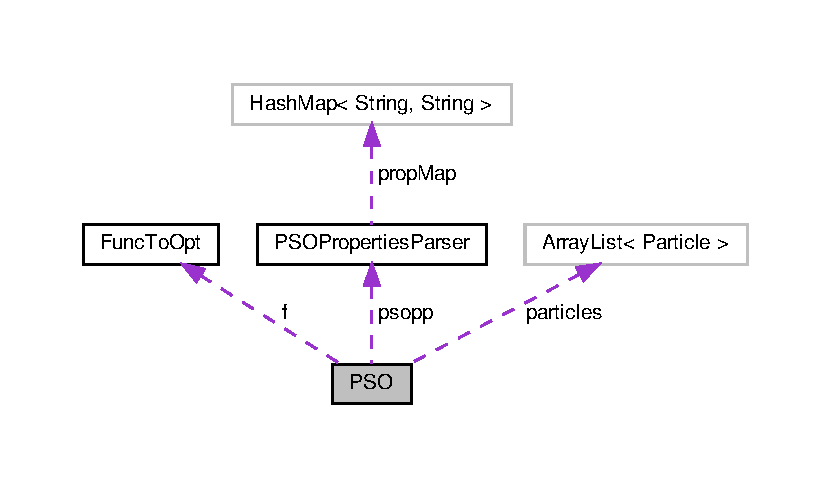
\includegraphics[width=350pt]{class_p_s_o__coll__graph}
\end{center}
\end{figure}
\subsection*{Public Member Functions}
\begin{DoxyCompactItemize}
\item 
\hyperlink{class_p_s_o_a0aeec4970276a5e318b613e8a192064e}{P\+SO} ()
\item 
void \hyperlink{class_p_s_o_ac3676d8b4b6eb1fcb0c05a14a20af85c}{add\+Particle} (\hyperlink{class_particle}{Particle} p)
\item 
\hyperlink{class_particle}{Particle} \hyperlink{class_p_s_o_a3c697a11238d768ae2b1236d3cf6ea88}{get\+Particle} (int i)
\item 
int \hyperlink{class_p_s_o_acc2a16aac995a30f3265fa06182509af}{get\+Num\+Particles} ()
\item 
int \hyperlink{class_p_s_o_a46ddfeb9df3a42b2f1b2c4fe0d8f51b2}{get\+Particles\+Dimension} ()
\item 
double \hyperlink{class_p_s_o_a57be39727a5a7e22182c82d4274ba3ae}{get\+Tol} ()
\item 
int \hyperlink{class_p_s_o_a0d3cd48e829ba5ccb754e26f1890e51b}{get\+Max\+Num\+Of\+Iterations} ()
\item 
double \hyperlink{class_p_s_o_a50f5f8be53be944150317d590c411144}{getW} ()
\item 
double \hyperlink{class_p_s_o_a51bdbe662e545c50ac984abdba9f6448}{get\+PhiP} ()
\item 
double \hyperlink{class_p_s_o_a9ddf1bc2e611d1959fe4f6fdef960b0e}{get\+PhiG} ()
\item 
double \mbox{[}$\,$\mbox{]} \hyperlink{class_p_s_o_af3fe18f93011219d7fc3badc9220b54b}{get\+Solution} ()
\item 
void \hyperlink{class_p_s_o_a83a2cd74d2176ea147b84e17050ceffb}{print\+Solution} ()
\item 
void \hyperlink{class_p_s_o_a689d26e00d138c809a4de0a34e98cd0a}{run} ()
\end{DoxyCompactItemize}
\subsection*{Static Public Member Functions}
\begin{DoxyCompactItemize}
\item 
static void \hyperlink{class_p_s_o_a966198c3d9ecb21acf593a5e922ba843}{main} (String\mbox{[}$\,$\mbox{]} args)
\end{DoxyCompactItemize}


\subsection{Constructor \& Destructor Documentation}
\mbox{\Hypertarget{class_p_s_o_a0aeec4970276a5e318b613e8a192064e}\label{class_p_s_o_a0aeec4970276a5e318b613e8a192064e}} 
\index{P\+SO@{P\+SO}!P\+SO@{P\+SO}}
\index{P\+SO@{P\+SO}!P\+SO@{P\+SO}}
\subsubsection{\texorpdfstring{P\+S\+O()}{PSO()}}
{\footnotesize\ttfamily P\+S\+O.\+P\+SO (\begin{DoxyParamCaption}{ }\end{DoxyParamCaption})}

Constructor. 

\subsection{Member Function Documentation}
\mbox{\Hypertarget{class_p_s_o_ac3676d8b4b6eb1fcb0c05a14a20af85c}\label{class_p_s_o_ac3676d8b4b6eb1fcb0c05a14a20af85c}} 
\index{P\+SO@{P\+SO}!add\+Particle@{add\+Particle}}
\index{add\+Particle@{add\+Particle}!P\+SO@{P\+SO}}
\subsubsection{\texorpdfstring{add\+Particle()}{addParticle()}}
{\footnotesize\ttfamily void P\+S\+O.\+add\+Particle (\begin{DoxyParamCaption}\item[{\hyperlink{class_particle}{Particle}}]{p }\end{DoxyParamCaption})}

Adds a new particle to the list of particles. 
\begin{DoxyParams}{Parameters}
{\em p} & the new particle. \\
\hline
\end{DoxyParams}
\mbox{\Hypertarget{class_p_s_o_a0d3cd48e829ba5ccb754e26f1890e51b}\label{class_p_s_o_a0d3cd48e829ba5ccb754e26f1890e51b}} 
\index{P\+SO@{P\+SO}!get\+Max\+Num\+Of\+Iterations@{get\+Max\+Num\+Of\+Iterations}}
\index{get\+Max\+Num\+Of\+Iterations@{get\+Max\+Num\+Of\+Iterations}!P\+SO@{P\+SO}}
\subsubsection{\texorpdfstring{get\+Max\+Num\+Of\+Iterations()}{getMaxNumOfIterations()}}
{\footnotesize\ttfamily int P\+S\+O.\+get\+Max\+Num\+Of\+Iterations (\begin{DoxyParamCaption}{ }\end{DoxyParamCaption})}

Returns the maximum number of iterations for the \hyperlink{class_p_s_o}{P\+SO} algorithm to terminate. \begin{DoxyReturn}{Returns}
the maximum number of iterations for the \hyperlink{class_p_s_o}{P\+SO} algorithm to terminate. 
\end{DoxyReturn}
\mbox{\Hypertarget{class_p_s_o_acc2a16aac995a30f3265fa06182509af}\label{class_p_s_o_acc2a16aac995a30f3265fa06182509af}} 
\index{P\+SO@{P\+SO}!get\+Num\+Particles@{get\+Num\+Particles}}
\index{get\+Num\+Particles@{get\+Num\+Particles}!P\+SO@{P\+SO}}
\subsubsection{\texorpdfstring{get\+Num\+Particles()}{getNumParticles()}}
{\footnotesize\ttfamily int P\+S\+O.\+get\+Num\+Particles (\begin{DoxyParamCaption}{ }\end{DoxyParamCaption})}

Returns the number of particles. \begin{DoxyReturn}{Returns}
the number of particles. 
\end{DoxyReturn}
\mbox{\Hypertarget{class_p_s_o_a3c697a11238d768ae2b1236d3cf6ea88}\label{class_p_s_o_a3c697a11238d768ae2b1236d3cf6ea88}} 
\index{P\+SO@{P\+SO}!get\+Particle@{get\+Particle}}
\index{get\+Particle@{get\+Particle}!P\+SO@{P\+SO}}
\subsubsection{\texorpdfstring{get\+Particle()}{getParticle()}}
{\footnotesize\ttfamily \hyperlink{class_particle}{Particle} P\+S\+O.\+get\+Particle (\begin{DoxyParamCaption}\item[{int}]{i }\end{DoxyParamCaption})}

Returns a particle from the list of particles. 
\begin{DoxyParams}{Parameters}
{\em i} & the index of the particle to return. \\
\hline
\end{DoxyParams}
\begin{DoxyReturn}{Returns}
the particle at the input index. 
\end{DoxyReturn}
\mbox{\Hypertarget{class_p_s_o_a46ddfeb9df3a42b2f1b2c4fe0d8f51b2}\label{class_p_s_o_a46ddfeb9df3a42b2f1b2c4fe0d8f51b2}} 
\index{P\+SO@{P\+SO}!get\+Particles\+Dimension@{get\+Particles\+Dimension}}
\index{get\+Particles\+Dimension@{get\+Particles\+Dimension}!P\+SO@{P\+SO}}
\subsubsection{\texorpdfstring{get\+Particles\+Dimension()}{getParticlesDimension()}}
{\footnotesize\ttfamily int P\+S\+O.\+get\+Particles\+Dimension (\begin{DoxyParamCaption}{ }\end{DoxyParamCaption})}

Returns the dimension of the particles. \begin{DoxyReturn}{Returns}
the dimension of the particles. 
\end{DoxyReturn}
\mbox{\Hypertarget{class_p_s_o_a9ddf1bc2e611d1959fe4f6fdef960b0e}\label{class_p_s_o_a9ddf1bc2e611d1959fe4f6fdef960b0e}} 
\index{P\+SO@{P\+SO}!get\+PhiG@{get\+PhiG}}
\index{get\+PhiG@{get\+PhiG}!P\+SO@{P\+SO}}
\subsubsection{\texorpdfstring{get\+Phi\+G()}{getPhiG()}}
{\footnotesize\ttfamily double P\+S\+O.\+get\+PhiG (\begin{DoxyParamCaption}{ }\end{DoxyParamCaption})}

Returns the phiG parameter. \begin{DoxyReturn}{Returns}
the phiG parameter. 
\end{DoxyReturn}
\mbox{\Hypertarget{class_p_s_o_a51bdbe662e545c50ac984abdba9f6448}\label{class_p_s_o_a51bdbe662e545c50ac984abdba9f6448}} 
\index{P\+SO@{P\+SO}!get\+PhiP@{get\+PhiP}}
\index{get\+PhiP@{get\+PhiP}!P\+SO@{P\+SO}}
\subsubsection{\texorpdfstring{get\+Phi\+P()}{getPhiP()}}
{\footnotesize\ttfamily double P\+S\+O.\+get\+PhiP (\begin{DoxyParamCaption}{ }\end{DoxyParamCaption})}

Returns the phiP parameter. \begin{DoxyReturn}{Returns}
the phiP parameter. 
\end{DoxyReturn}
\mbox{\Hypertarget{class_p_s_o_af3fe18f93011219d7fc3badc9220b54b}\label{class_p_s_o_af3fe18f93011219d7fc3badc9220b54b}} 
\index{P\+SO@{P\+SO}!get\+Solution@{get\+Solution}}
\index{get\+Solution@{get\+Solution}!P\+SO@{P\+SO}}
\subsubsection{\texorpdfstring{get\+Solution()}{getSolution()}}
{\footnotesize\ttfamily double \mbox{[}$\,$\mbox{]} P\+S\+O.\+get\+Solution (\begin{DoxyParamCaption}{ }\end{DoxyParamCaption})}

Returns the solution. \begin{DoxyReturn}{Returns}
the solution. 
\end{DoxyReturn}
\mbox{\Hypertarget{class_p_s_o_a57be39727a5a7e22182c82d4274ba3ae}\label{class_p_s_o_a57be39727a5a7e22182c82d4274ba3ae}} 
\index{P\+SO@{P\+SO}!get\+Tol@{get\+Tol}}
\index{get\+Tol@{get\+Tol}!P\+SO@{P\+SO}}
\subsubsection{\texorpdfstring{get\+Tol()}{getTol()}}
{\footnotesize\ttfamily double P\+S\+O.\+get\+Tol (\begin{DoxyParamCaption}{ }\end{DoxyParamCaption})}

Returns the tolerance for terminating the algorithm. \begin{DoxyReturn}{Returns}
the tolerance for terminating the algorithm. 
\end{DoxyReturn}
\mbox{\Hypertarget{class_p_s_o_a50f5f8be53be944150317d590c411144}\label{class_p_s_o_a50f5f8be53be944150317d590c411144}} 
\index{P\+SO@{P\+SO}!getW@{getW}}
\index{getW@{getW}!P\+SO@{P\+SO}}
\subsubsection{\texorpdfstring{get\+W()}{getW()}}
{\footnotesize\ttfamily double P\+S\+O.\+getW (\begin{DoxyParamCaption}{ }\end{DoxyParamCaption})}

Returns the inertia weight. \begin{DoxyReturn}{Returns}
the inertia weight. 
\end{DoxyReturn}
\mbox{\Hypertarget{class_p_s_o_a966198c3d9ecb21acf593a5e922ba843}\label{class_p_s_o_a966198c3d9ecb21acf593a5e922ba843}} 
\index{P\+SO@{P\+SO}!main@{main}}
\index{main@{main}!P\+SO@{P\+SO}}
\subsubsection{\texorpdfstring{main()}{main()}}
{\footnotesize\ttfamily static void P\+S\+O.\+main (\begin{DoxyParamCaption}\item[{String \mbox{[}$\,$\mbox{]}}]{args }\end{DoxyParamCaption})\hspace{0.3cm}{\ttfamily [static]}}

Starting point of the application. T\+O\+DO\+: To check and (possibly) refactor the following classes\+:
\begin{DoxyEnumerate}
\item \hyperlink{class_p_s_o}{P\+SO} 
\end{DoxyEnumerate}\mbox{\Hypertarget{class_p_s_o_a83a2cd74d2176ea147b84e17050ceffb}\label{class_p_s_o_a83a2cd74d2176ea147b84e17050ceffb}} 
\index{P\+SO@{P\+SO}!print\+Solution@{print\+Solution}}
\index{print\+Solution@{print\+Solution}!P\+SO@{P\+SO}}
\subsubsection{\texorpdfstring{print\+Solution()}{printSolution()}}
{\footnotesize\ttfamily void P\+S\+O.\+print\+Solution (\begin{DoxyParamCaption}{ }\end{DoxyParamCaption})}

Prints the solution. \mbox{\Hypertarget{class_p_s_o_a689d26e00d138c809a4de0a34e98cd0a}\label{class_p_s_o_a689d26e00d138c809a4de0a34e98cd0a}} 
\index{P\+SO@{P\+SO}!run@{run}}
\index{run@{run}!P\+SO@{P\+SO}}
\subsubsection{\texorpdfstring{run()}{run()}}
{\footnotesize\ttfamily void P\+S\+O.\+run (\begin{DoxyParamCaption}{ }\end{DoxyParamCaption})}

Runs the iterative \hyperlink{class_p_s_o}{P\+SO} procedure. 

The documentation for this class was generated from the following file\+:\begin{DoxyCompactItemize}
\item 
/home/asal/\+Desktop/staff/asal\+\_\+code/\+P\+S\+O/\hyperlink{_p_s_o_8java}{P\+S\+O.\+java}\end{DoxyCompactItemize}

\hypertarget{class_p_s_o_properties_parser}{}\section{P\+S\+O\+Properties\+Parser Class Reference}
\label{class_p_s_o_properties_parser}\index{P\+S\+O\+Properties\+Parser@{P\+S\+O\+Properties\+Parser}}


Collaboration diagram for P\+S\+O\+Properties\+Parser\+:\nopagebreak
\begin{figure}[H]
\begin{center}
\leavevmode
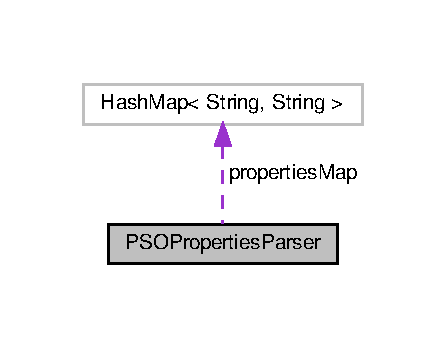
\includegraphics[width=214pt]{class_p_s_o_properties_parser__coll__graph}
\end{center}
\end{figure}
\subsection*{Public Member Functions}
\begin{DoxyCompactItemize}
\item 
void \hyperlink{class_p_s_o_properties_parser_a3165e06c1942985eaac001b29648b8c8}{read\+Properties\+Values} ()
\end{DoxyCompactItemize}


\subsection{Detailed Description}


Definition at line 8 of file P\+S\+O\+Properties\+Parser.\+java.



\subsection{Member Function Documentation}
\mbox{\Hypertarget{class_p_s_o_properties_parser_a3165e06c1942985eaac001b29648b8c8}\label{class_p_s_o_properties_parser_a3165e06c1942985eaac001b29648b8c8}} 
\index{P\+S\+O\+Properties\+Parser@{P\+S\+O\+Properties\+Parser}!read\+Properties\+Values@{read\+Properties\+Values}}
\index{read\+Properties\+Values@{read\+Properties\+Values}!P\+S\+O\+Properties\+Parser@{P\+S\+O\+Properties\+Parser}}
\subsubsection{\texorpdfstring{read\+Properties\+Values()}{readPropertiesValues()}}
{\footnotesize\ttfamily void P\+S\+O\+Properties\+Parser.\+read\+Properties\+Values (\begin{DoxyParamCaption}{ }\end{DoxyParamCaption})}

Reads the values of the properties from the properties file. 

Definition at line 15 of file P\+S\+O\+Properties\+Parser.\+java.



The documentation for this class was generated from the following file\+:\begin{DoxyCompactItemize}
\item 
/home/asal/\+Desktop/staff/asal\+\_\+code/\+P\+S\+O/\hyperlink{_p_s_o_properties_parser_8java}{P\+S\+O\+Properties\+Parser.\+java}\end{DoxyCompactItemize}

\chapter{File Documentation}
\hypertarget{_distance_calculator_8java}{}\section{/home/asal/\+Desktop/staff/asal\+\_\+code/\+P\+S\+O/\+Distance\+Calculator.java File Reference}
\label{_distance_calculator_8java}\index{/home/asal/\+Desktop/staff/asal\+\_\+code/\+P\+S\+O/\+Distance\+Calculator.\+java@{/home/asal/\+Desktop/staff/asal\+\_\+code/\+P\+S\+O/\+Distance\+Calculator.\+java}}
\subsection*{Classes}
\begin{DoxyCompactItemize}
\item 
class \hyperlink{class_distance_calculator}{Distance\+Calculator}
\end{DoxyCompactItemize}

\hypertarget{_func_to_opt_8java}{}\section{Func\+To\+Opt.\+java File Reference}
\label{_func_to_opt_8java}\index{Func\+To\+Opt.\+java@{Func\+To\+Opt.\+java}}
\subsection*{Classes}
\begin{DoxyCompactItemize}
\item 
class \hyperlink{class_func_to_opt}{Func\+To\+Opt}
\end{DoxyCompactItemize}

\hypertarget{_particle_8java}{}\section{Particle.\+java File Reference}
\label{_particle_8java}\index{Particle.\+java@{Particle.\+java}}
\subsection*{Classes}
\begin{DoxyCompactItemize}
\item 
class \hyperlink{class_particle}{Particle}
\end{DoxyCompactItemize}

\hypertarget{_p_s_o_8java}{}\section{/home/asal/\+Desktop/staff/asal\+\_\+code/\+P\+S\+O/\+P\+SO.java File Reference}
\label{_p_s_o_8java}\index{/home/asal/\+Desktop/staff/asal\+\_\+code/\+P\+S\+O/\+P\+S\+O.\+java@{/home/asal/\+Desktop/staff/asal\+\_\+code/\+P\+S\+O/\+P\+S\+O.\+java}}
\subsection*{Classes}
\begin{DoxyCompactItemize}
\item 
class \hyperlink{class_p_s_o}{P\+SO}
\end{DoxyCompactItemize}

\hypertarget{_p_s_o_properties_parser_8java}{}\section{P\+S\+O\+Properties\+Parser.\+java File Reference}
\label{_p_s_o_properties_parser_8java}\index{P\+S\+O\+Properties\+Parser.\+java@{P\+S\+O\+Properties\+Parser.\+java}}
\subsection*{Classes}
\begin{DoxyCompactItemize}
\item 
class \hyperlink{class_p_s_o_properties_parser}{P\+S\+O\+Properties\+Parser}
\end{DoxyCompactItemize}

\hypertarget{_r_e_a_d_m_e_8md}{}\section{/home/asal/\+Desktop/staff/asal\+\_\+code/\+P\+S\+O/\+R\+E\+A\+D\+ME.md File Reference}
\label{_r_e_a_d_m_e_8md}\index{/home/asal/\+Desktop/staff/asal\+\_\+code/\+P\+S\+O/\+R\+E\+A\+D\+M\+E.\+md@{/home/asal/\+Desktop/staff/asal\+\_\+code/\+P\+S\+O/\+R\+E\+A\+D\+M\+E.\+md}}

%--- End generated contents ---

% Index
\backmatter
\newpage
\phantomsection
\clearemptydoublepage
\addcontentsline{toc}{chapter}{Index}
\printindex

\end{document}
